%PDF DI RIFERIMENTO: 06_System Design.pdf + DesignPractices.pdf, 08_Architetture Software.pdf, 08_Architetture.pdf, XX-REST-APIs.pdf

\chapter{System Design}
    La progettazione del sistema è un insieme di scelte effettuate dall'ingegnere del software per la trasformazione del modello di analisi nel modello di design del sistema. \\
    Vengono qui definiti gli obiettivi di progettazione del software, l'architettura del sistema (il quale viene decomposto in più sottosistemi realizzabili da differenti squadre di sviluppatori) e le strategie di creazione del sistema.

    \section{Architettura e criteri di progettazione}
        L'architettura di un software è la struttura del sistema, che comprende gli elementi del software, le proprietà visibili all'esterno di tali elementi, e le relazioni tra di essi. \\
        Sulla base delle richieste avanzate dagli utenti, ovvero di un’applicazione \textbf{portabile}, \textbf{facile da usare} e \textbf{rapida}, si ritiene che i criteri di progettazione sui quali bisogni focalizzarsi siano \textbf{bassi tempi di risposta (bassa latenza)}, \textbf{basso consumo di memoria}, \textbf{alta portabilità e modificabilità}. \\
        Per soddisfare tali requisiti qualitativi, il sistema deve essere suddiviso in diversi moduli tali che tra essi sussistano un'\textbf{alta coesione} e un \textbf{basso accoppiamento}. \\
        Si è optato, in questo sistema, per un'\textbf{architettura client-server a due livelli con modello client leggero}. \\
        Si desidera ora evidenziare i criteri di progettazione definiti che hanno portato a questa decisione:
        \begin{itemize}
            \item La coesione è una misura di quanto siano fortemente relate e mirate le responsabilità, cioè i servizi offerti da un modulo; ciò permetterà di ottenere un’alta manutenibilità del codice e focalizzare i cambiamenti in interventi mirati e precisi. \\
            Per ottenere un'alta coesione, si è optato per una architettura client-server, nella quale ogni modulo adempie ad una funzione ben precisa e le cui classi collaborano per lo stesso fine. \\
            L'architettura client-server è una architettura distribuita, ove un sottosistema "servitore" offre servizi e dati ad altri sottosistemi "cliente", i quali sono responsabili dell'interazione con l'utente. \\
            I client chiamano il server richiedendo un servizio e ad essi viene restituito il risultato; questa chiamata è possibile poiché i client conoscono le interfacce del server, ma non è vero il viceversa.
            \item L’accoppiamento è una misura su quanto fortemente un modulo sia dipendente da altri. \\
            Un basso accoppiamento permetterà il riutilizzo dei moduli nonché una facilitazione nella modifica dello stesso, senza che le modifiche possano avere conseguenze inaspettate su altri moduli. \\
            Per ottenere un basso accoppiamento, si è scelto di seguire la legge di Demetra, spingendo al massimo l'incapsulamento.
            \item Il modello client leggero è l'alternativa al modello client pesante in un'architettura client-server a doppio legame. \\
            In questo modello, il client si occupa solamente dell'interfaccia e l'interazione con l'utente, e quindi può essere eseguito su gran parte dei dispositivi, anche con modeste prestazioni. \\
            Lo svantaggio di tale scelta è che pone maggior carico di elaborazione sia sul server, che si occupa della logica dell'applicazione e dell'immagazzinamento dei dati, sia sulla rete.
        \end{itemize}

    \section{Tecnologie adottate}
        Il client è un'applicazione per sistema operativo \textbf{Android}, scritta in linguaggio \textbf{Kotlin} e fa uso della libreria per la gestione delle immagini \textbf{Coil}. \\
        Il server si articola in:
        \begin{itemize}
            \item Un'applicazione \textbf{Java} salvata in un'immagine ed eseguita in un container del programma \textbf{Docker (Compose)}, installato su una macchina virtuale fornita da \textbf{AWS EC2}.
            \item Una base di dati relazionale \textbf{PostgreSQL}, al cui interno sono conservati tutti i dati dell'applicazione, eseguita anch'essa come immagine Docker sulla stessa macchina virtuale AWS EC2.
        \end{itemize}
        Le immagini sono archiviate nella macchina virtuale AWS EC2. \\
        Per lo scambio di messaggi tra client e server (attraverso le \textbf{REST API}), si utilizzano \textbf{Retrofit} su client e \textbf{Spring Framework} su server. \\

        \subsection{Android}
            \subsubsection{Cos'è Android? \cite{Wikipedia1}}
                Android è un sistema operativo gratuito ed open source, basato su una versione modificata del kernel Linux e di altri software open source. Creato originariamente per dispositivi touch come smartphone e tablet, è ora esteso a circa 2.5 miliardi di dispositivi \cite{Google1}, tra i quali anche smartwatch (Wear OS), smart TV (Android TV) e personal computer (questi ultimi utilizzano una versione modificata della distribuzione Gentoo Linux, chiamata Chrome OS, ma possono eseguire una macchina virtuale per utilizzare applicazioni Android). Il sistema operativo è correntemente sviluppato da Google.
            \begin{figure}[htbp!]
                \centering
                
\includegraphics[width=0.5\linewidth]{Immagini/System Design/Android.png}
                \caption{Logo di Android}
            \end{figure}
            \subsubsection{Perché Android?}
                Quasi tutti ormai posseggono uno smartphone. Ed essendo un sistema operativo così diffuso (conta circa il 69.94\% del mercato dei sistemi operativi per dispositivi mobili \cite{Statcounter1}) e disponibile su una grande varietà di dispositivi, Android è la scelta giusta per rendere l'applicazione disponibile quasi ovunque ed accessibile a chiunque.
                
        \subsection{Kotlin}
            \subsubsection{Cos'è Kotlin? \cite{Wikipedia2}}
                Kotlin è un linguaggio di programmazione multi-piattaforma, staticamente e fortemente tipizzato con inferenza di tipo, general purpose, multi-paradigma (orientato agli oggetti, imperativo, funzionale). Sviluppato da JetBrains, Kotlin è realizzato per essere interscambiabile con Java, poiché è interpretato da una macchina virtuale Java (JVM) che utilizza la libreria di classi Java standard. Ha pian piano soppiantato l'utilizzo di Java per la realizzazione di applicazioni Android ed è diventato nel 2019 il linguaggio primario e consigliato da Google per la realizzazione di esse.
            \begin{figure}[htbp!]
                \centering
                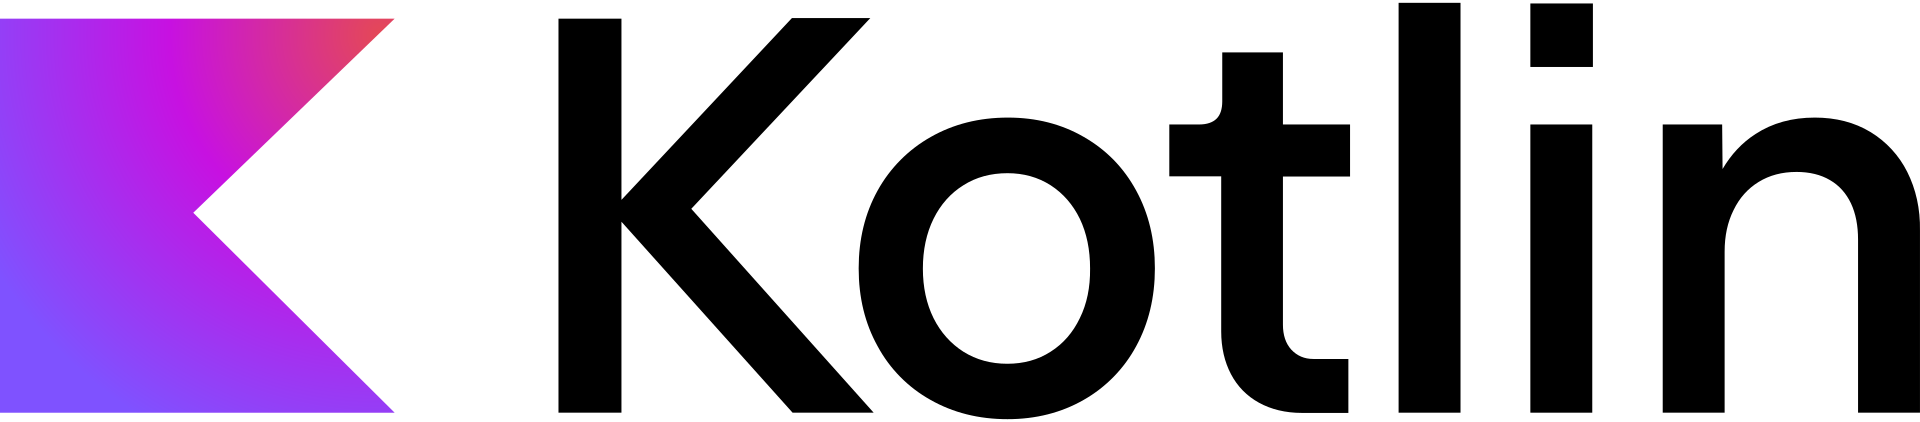
\includegraphics[width=0.5\linewidth]{Immagini/System Design/Kotlin.png}
                \caption{Logo di Kotlin}
            \end{figure}
            \subsubsection{Perché Kotlin? \cite{JetBrains1}}
                Circa il 50\% degli sviluppatori Android utilizza Kotlin (Java ricopre il 30\%), e il 70\% di essi afferma che lo sviluppo in Kotlin li abbia resi più produttivi. Lo sviluppo con Kotlin consente di beneficiare di:
                \begin{itemize}
                    \item Minore quantità di codice con conseguente maggiore leggibilità;
                    \item Minore quantità di errori comuni che potrebbero comportare il crash delle applicazioni (ad esempio la gestione della nullità dei riferimenti \cite{JetBrains2});
                    \item Supporto per la libreria Jetpack Compose per la costruzione di interfaccia utente delle applicazioni;
                    \item Supporto per lo sviluppo multi-piattaforma, poiché le librerie Kotlin possono essere utilizzabili anche per lo sviluppo di app iOS, desktop e web;
                    \item Maturità del linguaggio e dell'ambiente di sviluppo, continuamente migliorati e supportati;
                    \item Interoperabilità con Java, consentendo in iniettare codice Java in quello Kotlin e di utilizzare librerie di Java con Kotlin;
                    \item Semplicità e facilità di apprendimento ed utilizzo.
                \end{itemize}
                 
        \subsection{Coil}
            \subsubsection{Cosè Coil?}
                Coil (COroutine Image Loader) è una libreria per il caricamento delle immagini nelle app Android, scritta interamente in Kotlin, che permette di rendere semplici, rapidi ed indolori la visualizzazione delle immagini sull'interfaccia e la gestione in memoria delle stesse.
            \begin{figure}[htbp!]
                \centering
                
\includegraphics[width=0.5\linewidth]{Immagini/System Design/Coil.png}
                \caption{Logo di Coil}
            \end{figure}
            \subsubsection{Perché Coil? \cite{Github1}}
                Coil sfrutta le Coroutine Kotlin per assolvere al suo ruolo in maniera asincrona. Coil è:
                \begin{itemize}
                    \item Rapido, grazie a numerose operazioni di ottimizzazione quali cache in memoria e su archiviazione, sotto-campionamento delle immagini in memoria, gestione automatica delle richieste di pausa e cancellazione della visualizzazione ed altro;
                    \item Leggero, poiché aggiunge la quantità minima di metodi possibili per svolgere le sue funzioni;
                    \item Facile da usare, poiché sfrutta la semplicità di Kotlin e codice boilerplate minimale;
                    \item Moderno, perché sfrutta le più moderne librerie di Kotlin quali Coroutine, OkHttp, Okio, e Lifecycle AndroidX.
                \end{itemize}
                
        \subsection{Java}
            \subsubsection{Cos'è Java?}
                Java è un linguaggio di programmazione staticamente e fortemente tipizzato, general purpose, multi-paradigma (orientato agli oggetti, imperativo, funzionale). Sviluppato da Oracle, in precedenza Sun Microsystems, è un linguaggio interpretato e compilato. Il codice sorgente è compilato in un linguaggio intermedio chiamato bytecode che viene interpretato da una macchina virtuale Java (JVM).  Java è presente su miliardi di dispositivi in tutto il mondo.
            \begin{figure}[htbp!]
                \centering
                
\includegraphics[width=0.15\linewidth]{Immagini/System Design/Java.png}
                \caption{Logo di Java}
            \end{figure}
            \subsubsection{Perché Java?}
                Il fatto che Java sia un linguaggio eseguito su macchina virtuale comporta:
                \begin{itemize}
                    \item Sicurezza, perché ogni programma è isolato e ogni comunicazione con l'esterno è controllata dalla JVM, impedendo l'esecuzione di codice malizioso;
                    \item Portabilità, poiché il codice viene trasformato in un codice universalmente comprensibile da tutte le implementazioni della JVM sui vari dispositivi (PC, dispositivi mobili, dispositivi specializzati, server, workstation...);
                \end{itemize}
                Il linguaggio è anche open source e ampiamente utilizzato da milioni di sviluppatori nel mondo, e possiede una ricca libreria standard di funzioni per la realizzazione delle applicazioni. Infine, molti framework, tra i quali il selezionato Spring, si basano proprio su questo linguaggio.
                
        \subsection{Docker (Compose)}
            \subsubsection{Cos'è Docker (Compose)?}
                Docker è un insieme di servizi Platform as a Service (PaaS) che utilizza la virtualizzazione a livello di sistema operativo del kernel per eseguire programmi in ambienti isolati e distribuibili chiamati container, i quali sono gestiti dal Docker Engine \cite{Wikipedia5}. I container sono leggeri e al loro interno conterranno tutto il necessario per l'esecuzione del software, senza preoccuparsi di quale macchina sta eseguendo il Docker Engine. Questi container sono configurabili attraverso l'uso di file di configurazione appositi. Compose, inizialmente un add-on per la piattaforma Docker, è stato successivamente incluso al suo interno, e consente attraverso un singolo file YAML la gestione e la comunicazione reciproca di più container. I container sono un'istanza di un'immagine Docker, ossia un template di sola lettura che istruisce su come il container debba essere creato \cite{Docker1}.
            \begin{figure}[htbp!]
                \centering
                
\includegraphics[width=0.5\linewidth]{Immagini/System Design/Docker.png}
                \caption{Logo di Docker}
            \end{figure}
            \subsubsection{Perché Docker (Compose)?}
                Il successo di Docker è dovuto al rivoluzionario approccio allo sviluppo che esso promuove. Grazie a Docker, si può impacchettare all'interno di un'immagine Docker l'applicazione e tutto l'ambiente necessario alla sua esecuzione. L'immagine può essere caricata sulla repository centrale di Docker affinché chiunque possa accedervi, o comunque essere distribuita. Non bisogna quindi preoccuparsi di nulla: ogni container è isolato e contiene tutto ciò che è necessario, e non c'è bisogno di installare applicazioni oltre al Docker Engine, né gestire le librerie o le versioni dei linguaggi installati. Aggiornamenti dei software possono essere sempre rilasciati attraverso le immagini, e basta scaricarne la nuova versione e metterla in esecuzione sull'Engine per poter disporre degli ultimi strumenti. Permette anche di avere sulla stessa macchina più istanze in esecuzione di una stessa applicazione o servizio per favorire il bilanciamento del carico, la tolleranza al guasto e l'isolamento in caso di compromissione.
                
        \subsection{Google Cloud}
            \subsubsection{Cos'è Google Cloud?}
                Google Cloud Platform (GCP) è una suite di servizi di cloud computing offerta da Google che fornisce una enorme quantità di servizi cloud modulari, tra cui l'elaborazione, l'archiviazione dei dati, l'analisi dei dati e l'apprendimento automatico, insieme a una serie di strumenti di gestione. Esso è gestito con la stessa infrastruttura che Google utilizza internamente per i suoi prodotti per gli utenti finali. \cite{Wikipedia7} Nel contesto dell'applicazione DietiDeals24, sono stati utilizzati i servizi Artifact Registry per la conservazione delle immagini Docker, Cloud Build per la costruzione dei container a partire dalle immagini e Cloud Run per il deploy serverless del backend, Firebase per log e statistiche di utilizzo.
            \begin{figure}[htbp!]
                \centering
                
\includegraphics[width=0.5\linewidth]{Immagini/System Design/Google Cloud.png}
                \caption{Logo di Google Cloud}
            \end{figure}
            \subsubsection{Perché Google Cloud?}
                Google Cloud offre un'infrastruttura altamente scalabile, che consente alle aziende di crescere in modo efficiente. Possiede centri dati in tutto il mondo, garantendo bassa latenza ed alta disponibilità. Offre solide misure di sicurezza, tra cui crittografia dei dati, certificazioni di conformità e rilevamento avanzato delle minacce. Dispone di potenti strumenti di machine learning e AI che consentono analisi avanzate dei dati. Infine, con la tariffazione "pay-as-you-go", le aziende possono gestire i costi in modo efficace e pagare solo per ciò che utilizzano.

        \subsection{PostgreSQL}
            \subsubsection{Cos'è PostgreSQL? \cite{PostgreSQL1}}
                PostgreSQL è una potente base di dati relazionale gratuita ed open source che usa il linguaggio SQL standard ma non disdegnando delle aggiunte utili per conservare e scalare i carichi di dati più complessi (è gergalmente definito un "dialetto"). PostgreSQL ha una forte reputazione di RDBMS robusto, affidabile, estensibile. Esso è eseguibile su tutti i principali sistemi operativi e garantisce le proprietà ACID (atomicità, consistenza, isolamento, durabilità) per dati e transazioni. Inoltre fornisce anche utili add-on per estendere le capacità della base di dati. È disponibile sia attraverso riga di comando che GUI.
            \begin{figure}[htbp!]
                \centering
                
\includegraphics[width=0.2\linewidth]{Immagini/System Design/PostgreSQL.png}
                \caption{Logo di PostgreSQL}
            \end{figure}
            \subsubsection{Perché PostgreSQL?}
                PostgreSQL fornisce numerose funzionalità utili per lo sviluppo delle applicazioni, la protezione dell'integrità dei dati e la costruzione di ambienti tolleranti al guasto. Permette anche di scrivere procedure e funzioni procedurali in differenti linguaggi e per differenti linguaggi di programmazione (PL/pgSQL, PL/Tcl, PL/Perl, PL/Pyhton). Tra le funzionalità notevoli, si possono annoverare:
                \begin{itemize}
                    \item Supporto ad una vasta quantità di tipi di dato;
                    \item Funzionalità per il controllo dell'integrità dei dati;
                    \item Esecuzione concorrente e alte prestazioni;
                    \item Affidabilità e ripresa dal disastro;
                    \item Elevata sicurezza;
                    \item Ampia estensibilità;
                    \item Internazionalità e capacità di elaborazione testuale \cite{PostgreSQL1}; 
                    \item Supporto sempre gratuito;
                    \item Il linguaggio procedurale PL/pgSQL è pienamente compatibile con il linguaggio procedurale di altre basi di dati, facilitando eventuali future migrazioni \cite{Hevodata1}.
                \end{itemize}

        \subsection{REST API}
            \subsubsection{Cosa sono le REST API? \cite{IBM1}}
                Le REST API (REpresentational State Transfer Application Programming Interface) sono un'interfaccia di programmazione dell'applicazione che segue i princìpi REST, utilizzata per connettere tra loro componenti e applicazioni in un'architettura di microservizi. Le REST API sfruttano l'impalcatura del protocollo HTTP per poter permettere di effettuare tutte le principali operazioni sui dati attraverso i metodi HTTP, e i messaggi sono scambiati attraverso file JSON (ma anche XML o HTML).
            \subsubsection{Perché le REST API?}
                I sei princìpi REST sono un'interfaccia uniforme, il disaccoppiamento client-server, servizio senza stato, possibilità di utilizzo del meccanismo di cache, organizzazione del sistema a più livelli, ed esecuzione di codice su richiesta \cite{IBM1}. La realizzazione di applicazioni che comunicano attraverso REST API permette di spingere al massimo l'indipendenza tra i vari servizi, non rinunciando però ad una semplicità di fondo nella comunicazione, essendo il protocollo HTTP un protocollo maturo, quindi testato e funzionante, e strutturalmente semplice. Inoltre, la comunicazione attraverso file JSON (un formato comodo nella lettura sia per esseri umani che per calcolatori e uno dei formati di scambio dei dati più diffuso al mondo), ne permette la lettura da parte di moltissimi linguaggi di programmazione, ciascuno dei quali in possesso di strumenti di parsing di tale formato.

        \subsection{Retrofit}
            \subsubsection{Cos'è Retrofit?}
                Retrofit è un client HTTP type-safe per Android e Java sviluppato da Square. Semplifica il processo di interazione con i servizi web, consentendo agli sviluppatori di definire gli endpoint delle API mediante annotazioni e di eseguire le richieste di rete attraverso queste interfacce. Retrofit gestisce i dettagli delle richieste web, delle risposte e del parsing dei dati, facilitando l'integrazione delle API REST nelle applicazioni Android e Java.
            \begin{figure}[htbp!]
                \centering
                
\includegraphics[width=0.5\linewidth]{Immagini/System Design/Retrofit.png}
                \caption{Logo di Retrofit}
            \end{figure}
            
        \subsection{Spring Framework}
            \subsubsection{Cos'è Spring Framework?}
                Spring è un framework gratuito ed open source per applicazioni web scritte in Java. Inizialmente nato come alternativa al modello Enterprise JavaBeans di Java Enterprise Edition (ora Jakarta Enterprise Edition), le sue funzioni possono essere utilizzate da qualsiasi applicazione Java, e fornisce anche numerosi servizi aggiuntivi, che prendono il nome di Spring Boot, Spring Security, Spring Data, eccetera \cite{Wikipedia4}. Grazie a Spring, si possono realizzare delle REST API per la propria applicazione.
            \begin{figure}[htbp!]
                \centering
                
\includegraphics[width=0.5\linewidth]{Immagini/System Design/Spring.png}
                \caption{Logo di Spring}
            \end{figure}
            \subsubsection{Perché Spring Framework? \cite{Spoclearn1}}
                I punti forti di Spring sono:
                \begin{itemize}
                    \item Alta modularità e basso livello di dipendenze grazie al potente meccanismo di dependency injection, che promuove un basso accoppiamento, facilitando manutenzione e riusabilità;
                    \item  Ricco ecosistema, fornendo molti strumenti per ricoprire le varie necessità di sviluppo dell'applicazione;
                    \item Programmazione orientata all'aspetto, ossia permette di incapsulare le fasi più critiche dello sviluppo dell'applicazione, come la sicurezza e il tracciamento delle attività attraverso file di log;
                    \item Una community molto estesa e documentazione molto ampia;
                    \item Il supporto dello sviluppo orientato al test, assieme alla semplicità nella gestione delle dipendenza, contribuisce a migliori pratiche di test;
                    \item Flessibilità nella scelta di specifici componenti e moduli in base alle necessità del progetto.
                \end{itemize}